\documentclass[border=10pt]{standalone}
\usepackage{tikz}

\begin{document}

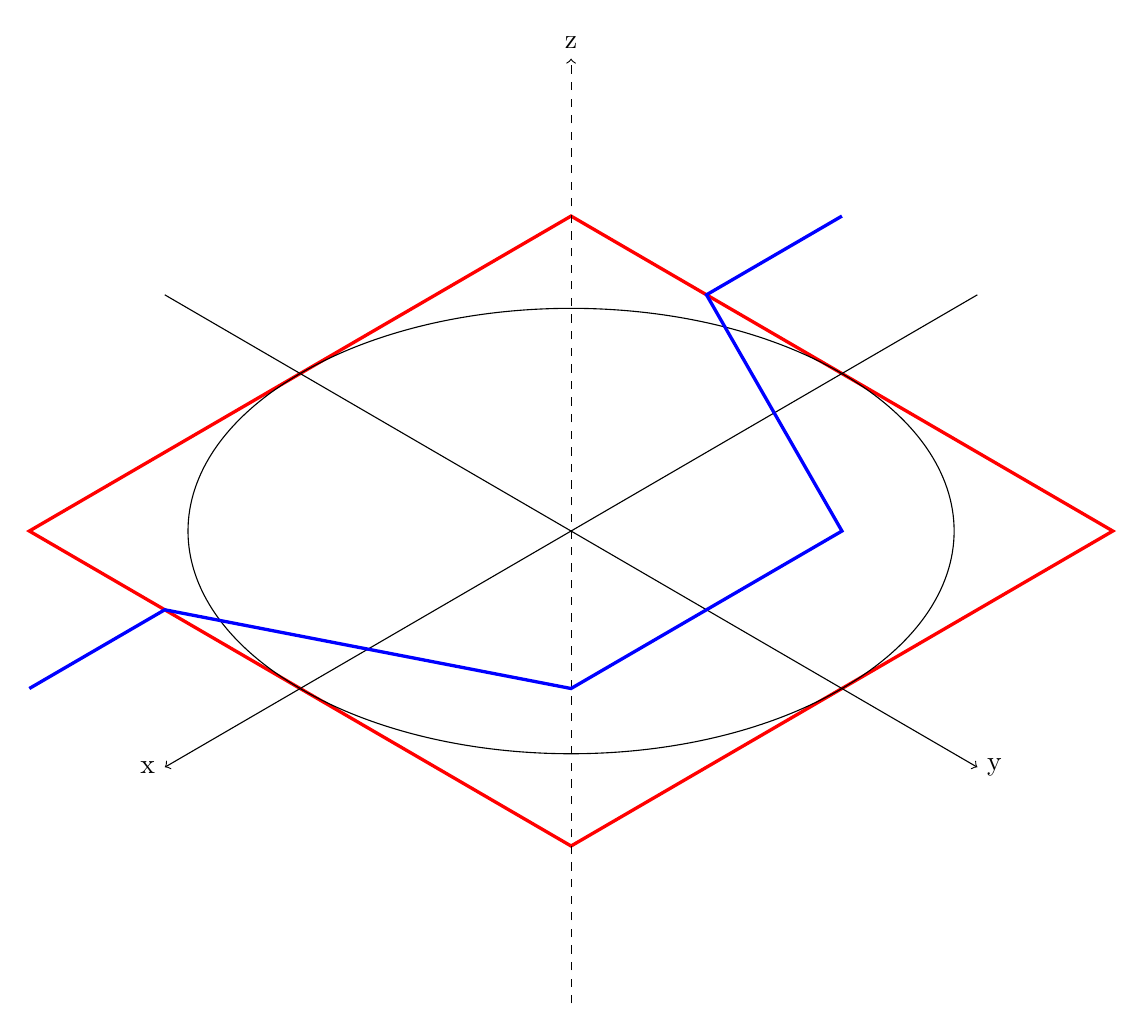
\begin{tikzpicture}[x={(-2*0.86cm,-2*0.5cm)}, y={(2*0.86cm,-2*0.5cm)}, z={(2*0cm,2*1cm)}]
    \draw[very thick, red] (-2,-2,0) -- (-2,2,0)-- (2,2,0) -- (2,-2,0) -- cycle;
    \draw[->] (-3,0,0) -- (3, 0,  0) node [left] {x};
    \draw[->] (0,-3,0) -- (0,  3, 0) node [right] {y};
    \draw[->,dashed] (0,0,-3) -- (0,  0, 3) node [above] {z};
    \draw circle (2);
    % \draw[very thick, blue] (-3,-1) -- +(1,0)-- +(2,2) -- +(4,2) -- +(5,0) -- +(6,0)-- cycle;
    % \draw[very thick, blue] (0,0,-4)+(-2,-2) circle(1) +(-2,2) circle (1) +(2,2) circle (1) +(2,-2) circle (1);
    \draw[very thick, blue] (-3,-1) -- ++(1,0)-- ++(1,2) -- ++(2,0) -- ++(1,-2) -- ++(1,0);

        
\end{tikzpicture}
\end{document}